%&"../ai"
\endofdump
\tikzexternalize[prefix=cache/]{hw02}
\begin{document}
    \title{第二次作业}
    \maketitle
    
    \begin{problem}
        尝试比较局部搜索算法(例如爬山法)与系统搜索算法(例如宽度优先搜索、A*算法)。
    \end{problem}

    \begin{problem}
        我们希望使用爬山法解决一些最优化问题。
        \begin{enumerate}
            \item 假设我们需要找$f(x,y,z) = e^x(xy+2z)$的最小值,且当前状态下我们有$(x,y,z) = (0,1,-1)$,那么我们需要将当前状态向怎样的方向进行移动、能够在理论上最快靠近极值?(方向用三维元组表示即可,计算过程可以参考多元函数的偏导数求解、最速下降法)。
            \item 使用爬山法搜索可能会遇到哪些问题?我们可以使用哪些更好的方法来代替?
        \end{enumerate}
    \end{problem}

    \begin{problem}
        我们的minimax搜索树如图\ref{hw2-figure1}所示。
        \begin{enumerate}
            \item 假如我们的\textbf{a}节点是\textbf{max}节点,请问最后\textbf{a}节点会得到怎样的值?
            \item 假如我们使用$\alpha-\beta$剪枝法进行minimax树的搜索,搜索过程中会从左至右访问相关节点,且\textbf{a}节点是\textbf{max}节点。算法运行过程中会访问多少个节点(包括字母标号的节点与数字标号的叶节点、忽略重复访问)?同时,请写下各节点的访问顺序(例如顺序:\textbf{"a - c - f - 43"})。
        \end{enumerate}
\begin{figure}[H]
  \centering
  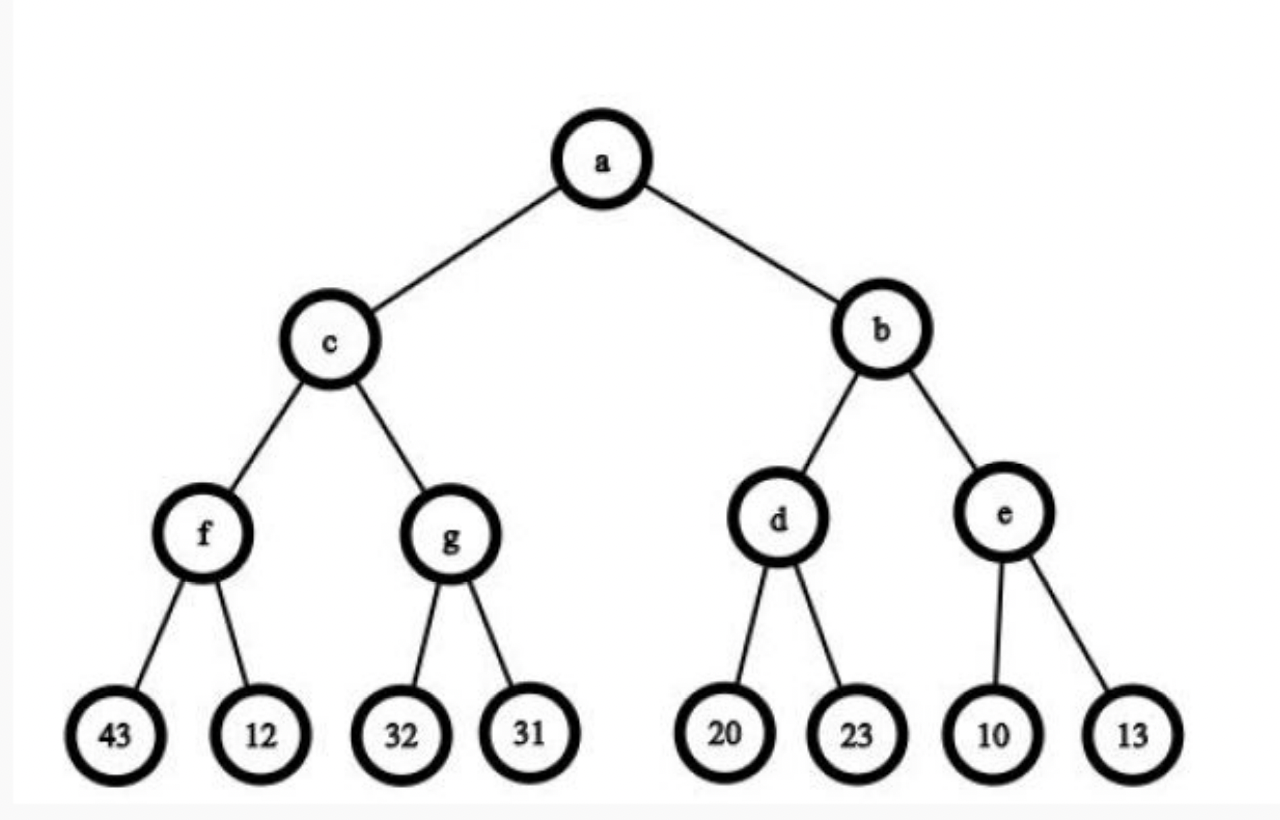
\includegraphics[width=0.8\linewidth]{hw2-figure1.png}
  \caption{第三题的对抗搜索树}
  \label{hw2-figure1}
\end{figure}
    \end{problem}

    \begin{problem}
        \indent 考虑一个这样的CSP问题:我们需要给变量\textit{$X_1, X_2, X_3, X_4$}赋值,需要满足以下约束:$(a)X_1\geq X_2, (b)X_2>X_3\ or\  X_3-X_2=2, (c)X_3\neq X_4, (d)X_1\neq X_3$。

\begin{figure}[H]
  \centering
  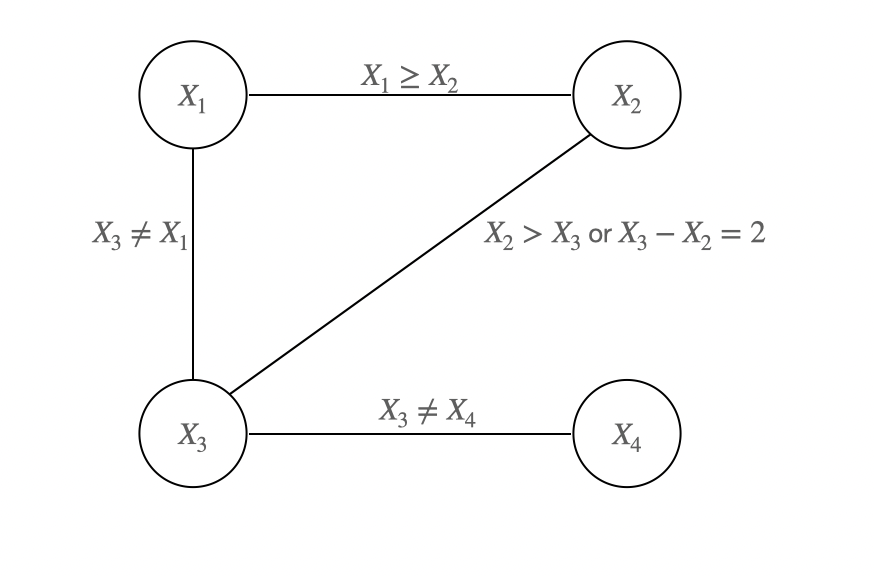
\includegraphics[width=0.5\linewidth]{hw2-figure2.png}
  \caption{第四题的csp问题}
  \label{hw2-figure2}
\end{figure}

\begin{enumerate}
    \item 根据CSP问题赋值求解的Most constraining variable规则,我们应该最先尝试给哪个变量赋值?
    \item 假如我们规定变量变量\textit{$X_1, X_2, X_3, X_4$}的值域分别为$D_1=\{1,2,3,4\}, D_2=\{3,4,5,8,9\}, D_3=\{2,3,5,6,7,9\}, D_4=\{3,5,7,8,9\}$。请问变量\textit{$X_1, X_2, X_3, X_4$}的哪些弧满足弧相容性(arc consistency)?
    \item 我们对该CSP问题在当前状态下运行AC3算法,请完成下方表格的步骤1-7。
\end{enumerate}

\begin{center}
初始的搜索列:$\{ X_2\rightarrow X_1$, $X_1\rightarrow X_2$, $X_3\rightarrow X_2$, $X_2\rightarrow X_3$, $X_4\rightarrow X_3$, $X_3\rightarrow X_4$, $X_3\rightarrow X_1$, $X_1\rightarrow X_3 \}$。\\
\begin{tabular}{|c|c|c|c|}
    \hline 
     步骤& 需要检查的弧$X_i\rightarrow X_j$ & $X_i$值域的变化 & 添加进入搜索列的弧   \\
     \hline 
     0 & $X_2\rightarrow X_1$ & 无变化  & 无 \\ \hline
     1 & $X_1\rightarrow X_2$ &  & \\ \hline
     2 & $X_3\rightarrow X_2$ &   &   \\ \hline
     3 & $X_2\rightarrow X_3$ &   &  \\ \hline
     4 & $X_4\rightarrow X_3$ &   &  \\ \hline
     5 & $X_3\rightarrow X_4$ &   &  \\ \hline
     6 & $X_3\rightarrow X_1$ &   &  \\ \hline
     7 & $X_1\rightarrow X_3$ &   & \\ \hline
     ...& ... & ... & \qquad \qquad \qquad \quad ... \\ \hline
\end{tabular}\\
\end{center}
    \end{problem}

\end{document}